\section{Literature Review}
% \textit{What is the problem to be solved, and it's significance?
% \begin{itemize}
%     \item Brief background to project
%     \item Summary of literature relevant to project
%     \item Identification of "gaps" in the literature
% \end{itemize}}

% The literature review is not just about presenting descriptions of the important papers you have found, but telling a meaningful story and, where appropriate, some critical discussion of previous findings (i.e. was another study useful but flawed?). Remember that you may read hundreds of papers/books/web pages etc., but often only about 20 or 30 are really important, and these are the ones you will mention in your literature review, which this report will be a concise version of. This section needs to flow logically, and this does not always imply that the material is chronological. By the end, the reader should have a clear appreciation of what the major work in the field was, why it is relevant to the current project, and where the unknowns and questions lie (\textbf{research gaps}) – these are the issues that you are going to address with your thesis research.

% For the purposes of this report, this section will be \textbf{12-15 pages long}. Remember to reference properly any material that you obtain from literature or other sources. If you are unsure how to discuss literature properly, find a really good review paper on your topic, or if there isn’t one, a similar topic, and you will have a good example to refer to.

\subsection{Principles of Photovoltaic Modules}
% Photovoltaic Module Definition
Photovoltaic modules, commonly known as solar panels, are devices that convert sunlight into electrical energy. \cite{EnelGreenPowerPhotovoltaicModule}\cite{U.S.DEPARTMENTofENERGY2024SolarBasics}\vspace{0.5em}

% Photoelectric Effect
Sunlight is made up of massless particles called photons, which possess a certain amount of energy. When these photons strike the surface, they knock electrons off of it, known as photoelectrons. This is known as the photoelectric effect, shown in Figure \ref{fig:photoelectric_effect_diagram}.\vspace{0.5em}

\begin{figure}[ht]
    \centering
    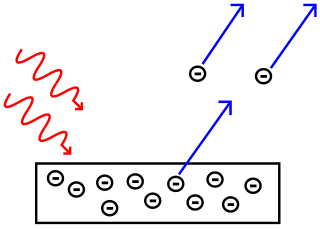
\includegraphics[width=0.4\textwidth]{Figures/photoelectric_effect_diagram.png}
    \caption{Photoelectric Effect Diagram. \cite{KhanAcademyPhotoelectricEffect}}
    \label{fig:photoelectric_effect_diagram}
\end{figure}
\FloatBarrier

The photoelectric effect will occur only if the frequency of the radiation is greater than the threshold frequency of the metal. The threshold frequency is the minimum frequency of light that causes electrons to be emitted from a material. The proportional relationship that exists between the threshold frequency and the work function is shown in Equation \ref{eq:work_function}.

\begin{equation}
    E = hf_0
    \label{eq:work_function}
\end{equation}

The work function refers to the minimum amount of energy needed to remove an electron from a metal surface. If photons with enough energy hit the surface, they can transfer their energy to the electrons allowing them to escape. If the energy of the incident photons is less than the work function, no electrons will be emitted, regardless of the intensity of the light. \cite{ScienceABC2023PhotoelectricBeginners}\vspace{0.5em}

% An Explanation of How Photovoltaic Modules Work
A photovoltaic module is made up of multiple photovoltaic cells, commonly known as solar cells. Each photovoltaic cell is made of semiconductor material, which is placed between the conductive layers. The most common semiconductor material used to make photovoltaic cells is silicon, accounting for 95 percent of photovoltaic modules sold worldwide. \cite{U.S.DEPARTMENTofENERGYSolarBasics} These photovoltaic cells use the photovoltaic effect to convert solar energy into electrical energy.\vspace{0.5em}

As shown in Figure \ref{fig:photovoltaic_cell_diagram}, a silicon photovoltaic cell is composed of two different layers of silicon: an n-type silicon layer, which has additional electrons, and a p-type silicon layer, which has extra spaces for the electrons, called holes.\vspace{0.5em}

\begin{figure}[ht]
    \centering
    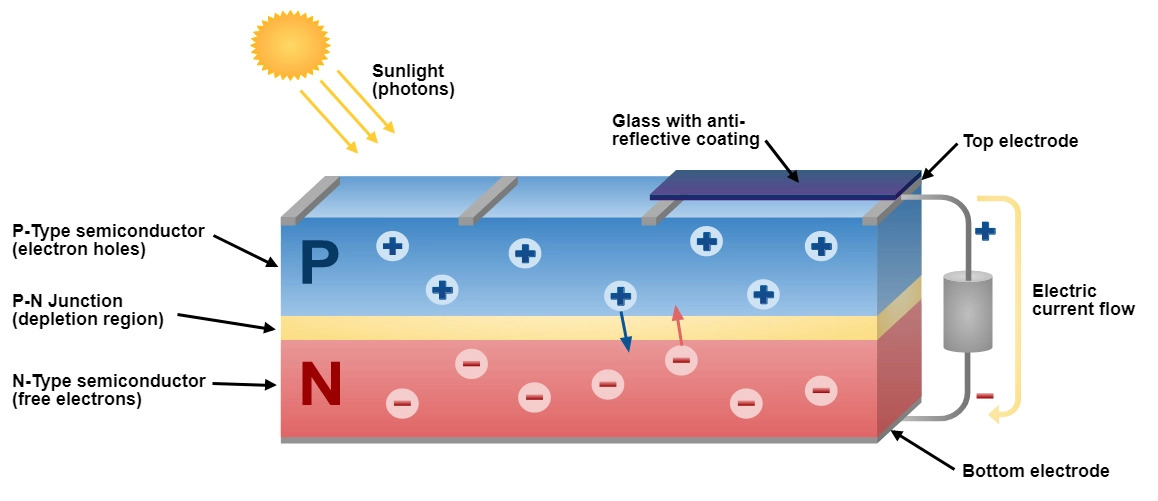
\includegraphics[width=1\textwidth]{Figures/photovoltaic_cell_diagram.jpg}
    \caption{Photovoltaic Cell Structure Diagram. \cite{Gupta2020SolarVehicle}}
    \label{fig:photovoltaic_cell_diagram}
\end{figure}
\FloatBarrier

When a proton strikes the silicon photovoltaic cell with the required energy, an electron is knocked out of its bond. Because of the electric field at the p-n junction, the negatively charged electron moves toward the n-side, while the resulting positively charged hole is attracted to the p-side. The free electrons are collected by thin metal fingers positioned at the top of the photovoltaic cell, before travelling through an external circuit. After electrical work is performed, the electrons are returned to the conductive aluminium sheet positioned at the back of the photovoltaic cell. Since electrons follow a continuous cycle and are the only moving components, there is no wear and tear, allowing photovoltaic cells to last for decades. \cite{TED-Ed2016HowKomp} However, they still have limitations.\vspace{0.5em}

\pagebreak
\subsection{Performance Limitations of Photovoltaic Modules}
A major limitation of photovoltaic modules is their declining electrical efficiency, particularly at high temperatures. A review led by Swapnil Dubey of Nanyang Technological University found that standard photovoltaic modules typically convert 6-20\% of incoming solar radiation into electrical energy. The remaining 80-94\% is mostly converted into heat, increasing the module’s temperature and further lowering its efficiency. \cite{Dubey2013TemperatureReview}\vspace{0.5em}

% An active cooling system for photovoltaic modules - H.G. Teo
A 2010 study led by H.G. Teo from the National University of Singapore refined Dubey et al.'s electrical efficiency range to 8-14\%. In the study, Teo et al. focused on comparing the electrical efficiency of photovoltaic modules under cooling and non-cooling conditions.\vspace{0.5em}

Teo et al. observed that the electrical efficiency of the photovoltaic module decreased as the temperature of the module increased, as shown in Figure \ref{fig:electrical_efficiency_vs_temperature_pv_module}. Teo et al. also found that without active cooling, the module temperature was significantly higher than when active cooling was applied under the same meteorological conditions. Thus, active cooling improved the module’s electrical efficiency from 8–9\% to 12–14\%. \cite{Teo2012AnModules}

\begin{figure}[ht]
    \centering
    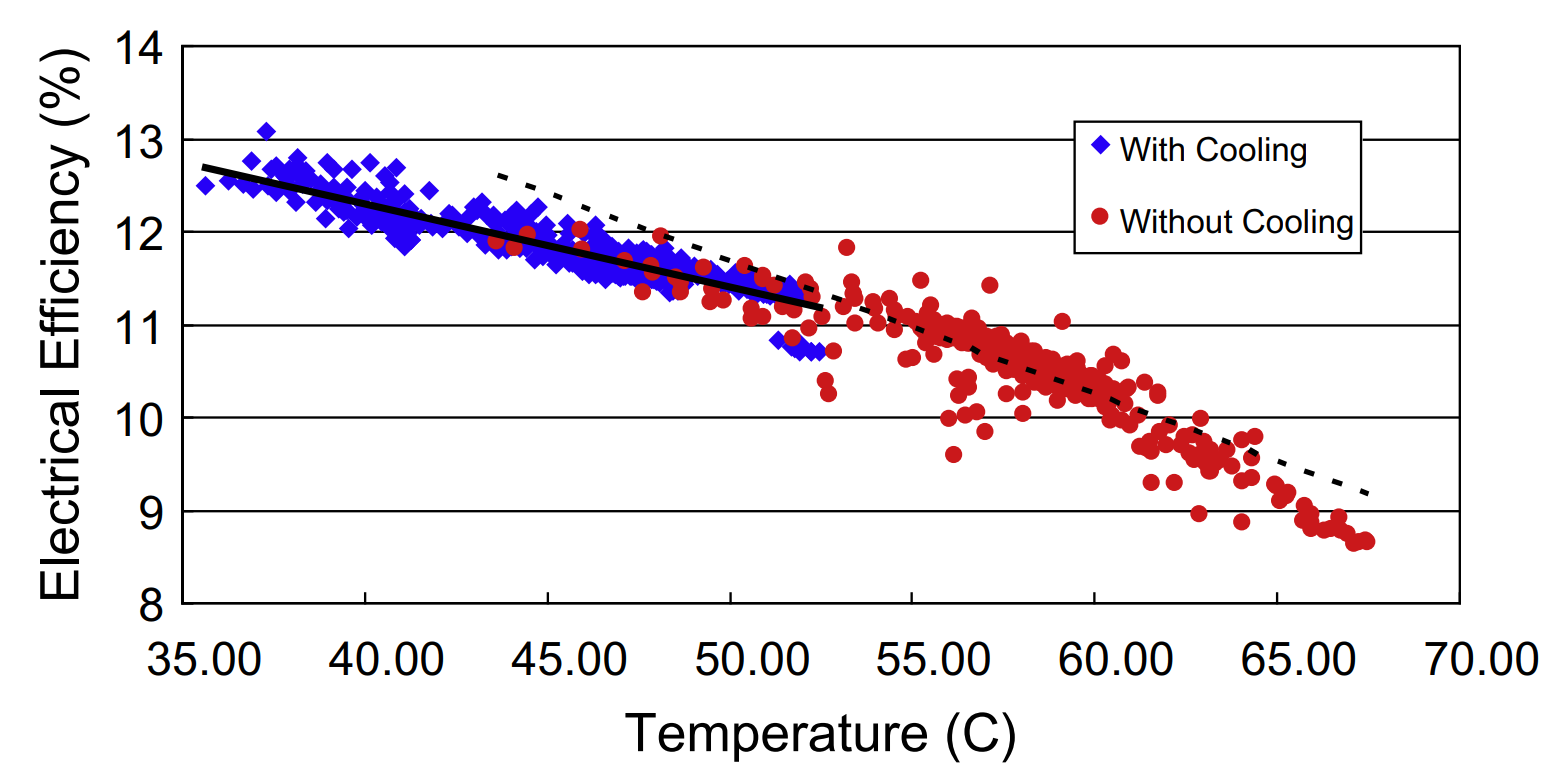
\includegraphics[width=0.7\textwidth]{Figures/electrical_efficiency_vs_temperature_pv_module.png}
    \caption{Electrical efficiency as a function of PV temperature. \cite{Teo2012AnModules}}
    \label{fig:electrical_efficiency_vs_temperature_pv_module}
\end{figure}
\FloatBarrier

The inverse linear relationship between the temperature and the electrical efficiency of a photovoltaic module is attributed to the band gap reduction, which occurs as the module's temperature increases.\vspace{0.5em}

% An explanation as to how increased module temperature leads to band gap reduction
In 1931, A.H. Wilson's paper, \textit{The Theory of Electronic Semi-Conductors}, introduced the idea that semiconductors have a small but finite band gap that affects their electrical conductivity. \cite{Il1931TheSemi-Conductors} The band gap represents the amount of energy that an electron must possess to jump from the valence band, where valence electrons are confined, to the conduction band. When valence electrons receive enough energy from an external source, they are able to undergo this band transition, which allows the material to conduct electricity. \cite{CircuitBread2018BandElectronics} As the temperature of the photovoltaic module increases, the valence electrons in the semiconductor material are excited. Thus, the energy required for an electron to transition from the valence band to the conduction band decreases, as indicated by a reduction in the band gap. \cite{Renewable_Tek2025HOTExplained}\vspace{0.5em}

% Electrical efficiency of a photovoltaic module
To understand the proportional relationship between the band gap and the electrical efficiency, an inspection of the formula used to calculate the electrical efficiency of a photovoltaic cell, shown in Equation \ref{eq:pv_cell_efficiency_function}, is required. \cite{HonsbergSolarEfficiency}

\begin{equation}
    \eta = \frac{V_\text{OC}I_\text{SC}FF}{P_\text{in}}
    \label{eq:pv_cell_efficiency_function}
\end{equation}

The open circuit voltage, short circuit current and fill factor are all affected by the band gap. Therefore, an investigation into the effect of a reduced band gap on these aforementioned variables is necessary to evaluate the impact that the band gap has on the electrical efficiency of the photovoltaic module.\vspace{0.5em}

% Open circuit voltage
A 1994 study led by P. Baruch from the University of Paris derived a formula for determining the minimum value of the diode saturation current, as shown in Equation \ref{eq:minimum_diode_saturation_current}.

\begin{equation}
    J_0 = \frac{q}{k} \frac{15\sigma}{\pi^4} T^3 \int_{u}^{\infty} \frac{x^2}{e^x - 1}\,dx
    \label{eq:minimum_diode_saturation_current}
\end{equation}

where $u = \frac{E_G}{kT}$. \cite{Baruch1995OnConversion} A casual inspection of Equation \ref{eq:minimum_diode_saturation_current} shows a relationship between the band gap energy and the diode saturation current. However, it is not immediately obvious what the nature of the relationship is due to the complexity of the integral function.\vspace{0.5em}

Just over a decade later, Michael Y. Levy and Christiana Honsberg from the University of Delaware proposed a method to evaluate the integral in Baruch's formula. \cite{Levy2006RapidApplications} Then, in 2017, Honsberg worked with Stuart Bowden to graph the relationship between the diode saturation current and the band gap based on this method, as shown in Figure \ref{fig:diode_saturation_current_bandgap_graph}.

\begin{figure}[ht]
    \centering
    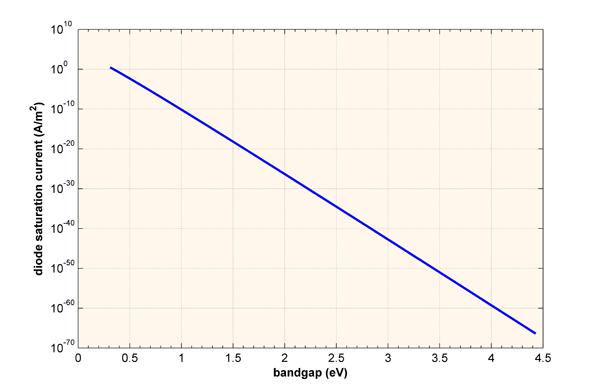
\includegraphics[width=0.7\textwidth]{Figures/diode_saturation_current_bandgap_graph.png}
    \caption{Diode saturation current as a function of band gap. The values are determined from detailed balance and place a limit on the open circuit voltage of a solar cell. \cite{HonsbergOpen-CircuitVoltage}}
    \label{fig:diode_saturation_current_bandgap_graph}
\end{figure}
\FloatBarrier

Honsberg and Bowden used the diode saturation current values, $J_0$, from Figure \ref{fig:diode_saturation_current_bandgap_graph}, denoted as $I_0$ in Equation \ref{eq:open_circuit_voltage_function}, to calculate the open-circuit voltage as a function of the band gap. The linearly proportional relationship between the band gap and the open-circuit voltage is shown in Figure \ref{fig:open-circuit_voltage_bandgap_graph}.

\begin{equation}
    V_{OC} = \frac{n k T}{q} \times \ln\left(\frac{I_L}{I_0} + 1\right)
    \label{eq:open_circuit_voltage_function}
\end{equation}

\begin{figure}[ht]
    \centering
    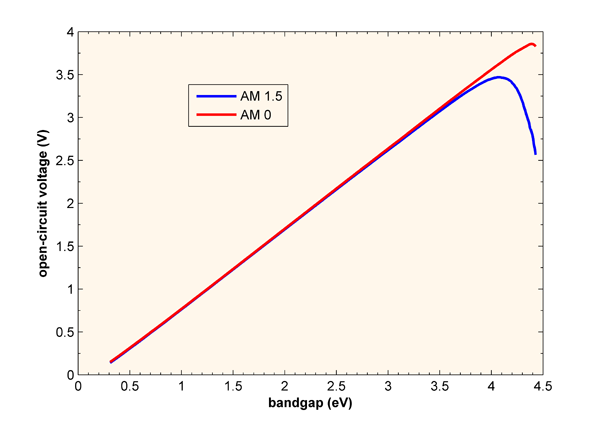
\includegraphics[width=0.7\textwidth]{Figures/open-circuit_voltage_bandgap_graph.png}
    \caption{$V_\text{OC}$ as a function of band gap for a cell with AM 0 and AM 1.5. The $V_\text{OC}$ increases with bang gap as the recombination current falls. There is drop off in $V_\text{OC}$ at very high band gaps due to the very low $I_\text{SC}$. \cite{HonsbergOpen-CircuitVoltage}}
    \label{fig:open-circuit_voltage_bandgap_graph}
\end{figure}
\FloatBarrier

Thus, the reduced band gap due to the increased temperature of the photovoltaic module leads to a decrease in the open-circuit voltage. \cite{HonsbergOpen-CircuitVoltage}\vspace{0.5em}

\pagebreak
% Short circuit current
Honsberg and Bowden also graphed the relationship between the band gap and the short circuit current density, as shown in Figure \ref{fig:short_circuit_current_density_bandgap_graph}.

\begin{figure}[ht]
    \centering
    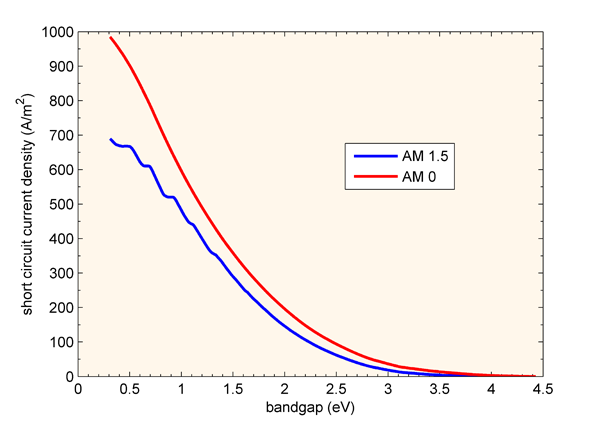
\includegraphics[width=0.7\textwidth]{Figures/short_circuit_current_density_bandgap_graph.png}
    \caption{$J_\text{SC}$ as a function of band gap for a cell with AM 0 and AM 1.5. \cite{HonsbergShort-CircuitCurrent}}
    \label{fig:short_circuit_current_density_bandgap_graph}
\end{figure}
\FloatBarrier

From Figure \ref{fig:short_circuit_current_density_bandgap_graph}, it is evident that a band gap reduction corresponds to an increase in the short circuit current density. Equation \ref{short_circuit_current_function} shows a linearly proportional relationship between the short circuit current and the short circuit current density.

\begin{equation}
    I_\text{SC} = J_\text{SC}A
    \label{short_circuit_current_function}
\end{equation}

Therefore, a decrease in the band gap leads to an increase in the short-circuit current. \cite{HonsbergShort-CircuitCurrent}\vspace{0.5em}

% Fill Factor
In 1981, M.A. Green of the University of New South Wales proposed an empirical expression for the fill factor, as shown in Equation \ref{eq:fill_factor_function}.

\begin{equation}
    FF = \frac{v_\text{OC} - ln(v_\text{OC} + 0.72)}{v_\text{OC} + 1}
    \label{eq:fill_factor_function}
\end{equation}

where $v_\text{OC}$ is defined as a normalised $V_\text{OC}$: $v_\text{OC} = \frac{q}{nkT} V_\text{OC}$. \cite{Green1981SolarExpressions}\vspace{0.5em}

As established earlier in Figure \ref{fig:open-circuit_voltage_bandgap_graph}, a band gap reduction corresponds to a decrease in the open-circuit voltage. An evaluation of Equation \ref{eq:fill_factor_function} reveals that a decline in the open-circuit voltage and an increase in the temperature of the photovoltaic module causes a decrease in the fill factor. Therefore, it can be concluded that a band gap reduction causes a decrease in the fill factor.\vspace{0.5em}

% Resultant conclusion
To summarise, the band gap reduction that arises due to the increased temperature of the photovoltaic module causes a decrease in the open-circuit voltage, an increase in the short circuit current and a decrease in the fill factor. While the short circuit current does increase, it is ultimately outweighed by the decrease in the open-circuit voltage and fill factor, leading to a decrease in the module's electrical efficiency.\vspace{0.5em}

% Additional factors
In addition to temperature, other environmental factors like shade and air pollution limit the electrical efficiency of photovoltaic modules. A 2013 study led by Alberto Dolara from the Polytechnic University of Milan found that shade significantly affects the performance of photovoltaic modules. Dolara et al. observed a 31\% drop in the power generated by a single photovoltaic cell when 50\% of the cell was subjected to shade. \cite{Dolara2013ExperimentalModules} In 2001, E. Asl-Soleimani et al. from the University of Tehran concluded that air pollution also reduced the energy output of photovoltaic modules by up to 60\%. \cite{Asl-Soleimani2001TheTehran} Furthermore, operational factors like poor module maintenance can lead to dust buildup, significantly reducing power generation. A review led by Khaled Hasan in 2021 stated a 60-70\% reduction in power generation due to the deposition of dust in humid conditions. \cite{Hasan2022EffectsReview} \vspace{0.5em} 

% Link the heat transfer paragraphs to the limitations paragraphs
In 1961, William Shockley and Hans Queisser published their paper, \textit{Detailed Balance Limit of Efficiency of p-n Junction Solar Cells}, in which they established the theoretical maximum efficiency of silicon-based solar cells to be approximately 30\% under standard illumination conditions. \cite{Shockley1961DetailedCells} In the real world however, photovoltaic cells are prevented from reaching this limit due to the environmental and operational factors previously discussed. Thus, due to the important role that photovoltaic modules play in the future of global energy, methods to reduce the impact that these factors have on the performance of photovoltaic modules are constantly being investigated. In particular, to mitigate the reduction in electrical efficiency caused by increased photovoltaic module temperature, heat transfer-based cooling methods are investigated and employed worldwide.\vspace{0.5em}

\pagebreak
\subsection{Heat Transfer in Photovoltaic Modules}
The fundamental concept of heat transfer is the process by which heat energy moves from one system or body to another as a result of a temperature difference. This transfer of heat can occur via conduction, convection or radiation. Figure \ref{fig:fundamental_concept_of_heat_transfer_diagram} demonstrates the fundamental concept of heat transfer in the context of a photovoltaic module.\vspace{0.5em}

\begin{figure}[h]
    \centering
    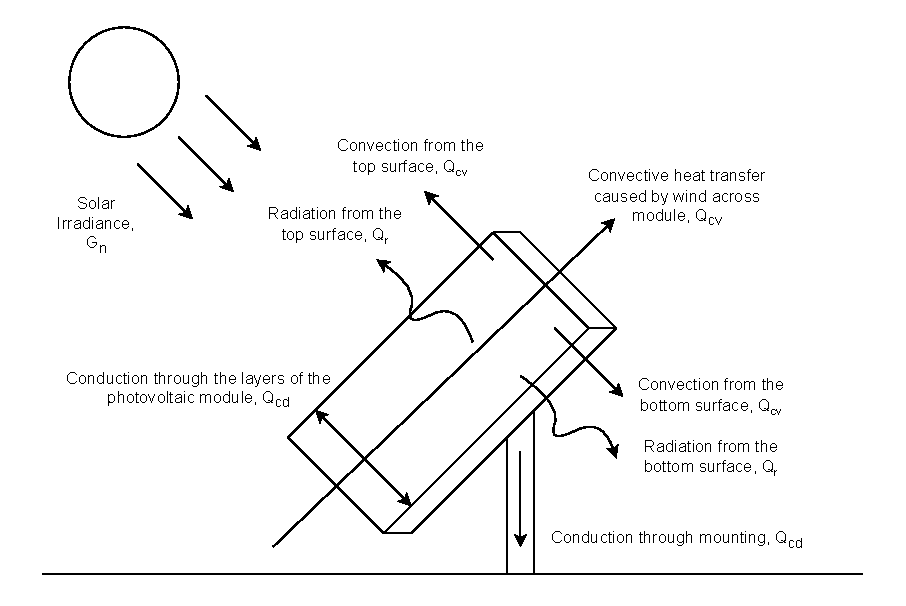
\includegraphics[width=0.75\textwidth]{Figures/fundamental_concept_of_heat_transfer_diagram.pdf}
    \caption{Fundamental concept of heat transfer on a photovoltaic module. Adapted from \cite{HonsbergHeatModules}}
    \label{fig:fundamental_concept_of_heat_transfer_diagram}
\end{figure}

In Figure \ref{fig:fundamental_concept_of_heat_transfer_diagram}, conductive heat transfer through the layers of the photovoltaic module and the mounting are observed. Additionally, heat is transferred from the surface of the photovoltaic module to the surrounding air via convection. Finally, the module emits thermal radiation to its surroundings, contributing to radiative heat transfer. In 2020, P. Dwivedi from the Maulana Azad National Institute of Technology, Bhopal, analysed the percentage distribution of heat loss across the different modes of heat transfer, shown in Table \ref{tab:heat_loss_from_pv_module}. \cite{Dwivedi2020AdvancedArt}

\begin{table}[ht]
    \centering
    \caption{Heat loss from P.V. module. \cite{Dwivedi2020AdvancedArt}}
    \setlength{\tabcolsep}{50pt} % Adjust column spacing between columns
    \renewcommand{\arraystretch}{1.5} % Increase row height
    \begin{tabular}{@{\hspace{8pt}} l l l @{\hspace{8pt}}}
         \hline
         S.No & Heat loss from module & Percentage \\
         \hline
         1 & Conduction through mounting & 2 \\
         2 & Convection from top surface & 42 \\
         3 & Convection from bottom surface & 24 \\
         4 & Radiation from top surface & 21 \\
         5 & Radiation from bottom surface & 11 \\
         \hline
    \end{tabular}
    \label{tab:heat_loss_from_pv_module}
\end{table}

An inspection of Table \ref{tab:heat_loss_from_pv_module} reveals that convection based heat transfer is the dominant form of heat transfer for photovoltaic modules.\par
Therefore, an identical percentage increase in rate of convective heat transfer will have a greater effect on the overall module heat transfer than the same increase in conductive or radiative heat transfer.\par
Thus, the following subsections will explore the effectiveness of conduction, convection, and radiation-based cooling methods in lowering the temperature of photovoltaic modules to enhance their overall efficiency with a focus on convection based cooling methods.\vspace{0.5em}
% An inspection of Table \ref{tab:heat_loss_from_pv_module} reveals that convective heat transfer is the dominant mode of thermal energy loss in photovoltaic modules.\par
% As a result, a given percentage increase in convective heat transfer will have a more significant impact on the total heat dissipation compared to an equivalent increase in conductive or radiative transfer.\par
% Therefore, the following subsections will evaluate the effectiveness of conduction-, convection-, and radiation-based cooling strategies in reducing the operating temperature of photovoltaic modules, with particular emphasis on convection-based methods due to their greater potential for improving overall efficiency.


\subsubsection{Conduction}
Conduction is the transfer of energy from the more energetic particles of a substance to the adjacent less energetic ones as a result of interactions between the particles. The formula commonly used to calculate the rate of heat conduction is shown in Equation \ref{eq:rate_of_heat_conduction_function}. \cite{Cengel2014IntroductionConcepts}

\begin{equation}
    \dot{Q}_\text{cond} = -kA\frac{\Delta T}{\Delta x}
    \label{eq:rate_of_heat_conduction_function}
\end{equation}

The main conduction-based cooling methods used to reduce photovoltaic module temperatures are finned heat sinks and phase change materials.\vspace{0.5em}

% Finned Heat Sinks
A heat sink is a component used in thermal management strategies to transfer heat effectively. It's design is optimised to dissipate heat. \cite{Kumar2024QualitativeReview} The use of a heat sink increases the cross-sectional area that the heat is being transferred to, denoted as $A$ in Equation \ref{eq:rate_of_heat_conduction_function}. Through further inspection of Equation \ref{eq:rate_of_heat_conduction_function}, it is observed that the increased cross-sectional area, $A$, results in an increased rate of conductive heat transfer, $\dot{Q}_\text{cond}$. A study led by S.N. Razali from the National University of Malaysia investigated the effect of multidirectional tapered fin heat sinks (MTFHS) on photovoltaic modules. Razali et al. found that the proposed MTFHS reduced the module's temperature by $12^\circ \text{C}$, indicating enhanced conductive heat transfer, which consequently improved the photovoltaic module's efficiency by 1.53\% \cite{Razali2023PerformanceMTFHS}.\vspace{0.5em}

% Phase Change Materials 
A phase change material (PCM) is a material that can change its state from solid to liquid and vice versa by releasing and storing thermal energy. \cite{Nicholas2019ActivatedMaterial} When the surrounding temperature rises above the PCM’s melting point, it liquefies, drawing heat away from the photovoltaic module. Conversely, when the temperature drops below the melting point, the PCM solidifies, releasing the stored heat back into the environment. A 2023 study by B. Hussain and colleagues at the Capital University of Science \& Technology found that incorporating PCM lowered the surface temperature of photovoltaic modules by $13.1^\circ \text{C}$, resulting in a 6.85\% increase in efficiency. \cite{Hussain2023Phase}\vspace{0.5em}

% Limitations of Conduction Based Cooling Methods
While conduction-based cooling methods have been successful in improving photovoltaic module efficiency, they do have certain limitations.\par
\par

\subsubsection{Radiation}
Radiation is the energy emitted by matter in the form of electromagnetic waves (or photons) due to changes in the electronic configurations of the atoms or molecules. In the context of heat transfer, the focus is on thermal radiation, which is the energy emitted by bodies due to their temperature. The formula commonly used to calculate the rate of radiation heat transfer is shown in Equation \ref{eq:rate_of_heat_radiation_function}. \cite{Cengel2014IntroductionConcepts}

\begin{equation}
    \dot{Q}_\text{rad} = \varepsilon\sigma A_s (T_s^4-T_\text{surr}^4)
    \label{eq:rate_of_heat_radiation_function}
\end{equation}

% polydimethylsiloxane film
In 2018, a study led by B. Zhao from the University of Science and Technology of China investigated the performance impact of radiation-based cooling methods on photovoltaic modules. Zhao et al. modified a photovoltaic module by adding a polydimethylsiloxane (PDMS) film on its top surface. PDMS is known to have high emissivity in the mid-infrared range ($8-13\,\mu m$). \cite{Song2020UltrahighRegime} Through an inspection of Equation \ref{eq:rate_of_heat_radiation_function}, it is observed that an increased emissivity, $\varepsilon$, causes an increase in the rate of radiative heat transfer, $\dot{Q}_\text{rad}$. In theory, the increased radiative heat transfer of the photovoltaic module lowers the module's temperature and improves it's efficiency. However, Zhao et al. found that the temperature of the photovoltaic module was only reduced by 1.75 K in the ideal case. Furthermore, this result was achieved using a simulated environment. Thus, Zhao's team concluded that, in practical applications, enhanced radiative cooling does not offer significant potential for cooling photovoltaic modules. \cite{Zhao2018PerformanceModule}

% Limitations of Radiation Based Cooling Methods

\subsubsection{Convection}
% \textit{\textbf{I am unsure where to put laminar and turbulent flow}}\par
Convection is the mode of energy transfer between a solid surface and the adjacent liquid or gas that is in motion. The formula commonly used to calculate the rate of convective heat transfer can be expressed by Newton's law of cooling, shown in Equation \ref{eq:rate_of_convective_heat_transfer_function}. \cite{Cengel2014IntroductionConcepts}

\begin{equation}
    \dot{Q}_\text{conv} = hA_s(T_s-T_\infty)
    \label{eq:rate_of_convective_heat_transfer_function}
\end{equation}

Convection is not a fundamental heat transfer mechanism; rather, it is a combined phenomenon, where heat conduction occurs in the presence of fluid motion. Convection can be broadly categorised into two types: natural convection, also referred to as free convection, and forced convection. \cite{Cengel2014FundamentalsConvection}

\subsubsubsection{Natural Convection and Relevant Cooling Methods}
Natural convection is the process by which heat transferred to a fluid raises its temperature, reducing its density and generating buoyant forces. These forces cause the warmer, lighter fluid to rise, carrying the absorbed heat to another location where it can be dissipated. \cite{Zohuri2020ThermosyphonApplications} Figure \ref{fig:cooling_of_boiled_egg_natural_convection} illustrates natural convective heat transfer in the context of cooling a hot egg.

\begin{figure}[ht]
    \centering
    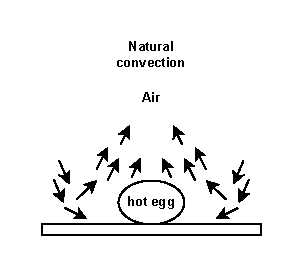
\includegraphics[width=0.5\textwidth, trim=0 10 0 15, clip]{Figures/cooling_of_boiled_egg_natural_convection.pdf}
    \caption{The cooling of a boiled egg by natural convection. Adapted from \cite{Cengel2014IntroductionConcepts}}
    \label{fig:cooling_of_boiled_egg_natural_convection}
\end{figure}

% RCM: Tilt angle optimization
The tilt angle of a photovoltaic module significantly influences natural convective heat transfer, as it alters the buoyancy-driven airflow around the module’s surface.\vspace{0.5em}

% \textit{\textbf{Talk about free convection boundary layers here}}\vspace{0.5em}

A 2021 study led by A. Abdulmunem from the University of Malaya, Malaysia, investigated the impact of tilt angle on the performance of photovoltaic systems. Abdulmunem et al. observed that as the tilt angle increased from $0^\circ$ (horizontal) to $90^\circ$ (vertical), the temperature reduction in the photovoltaic cell increased from $-0.4\%$ to $-12\%$. This trend was attributed to enhanced natural convective heat transfer which acts to improve photovoltaic module efficiency. Consequently, Abdulmunem et al. concluded that increasing the tilt angle of the photovoltaic module away from the horizontal axis and towards the vertical axis improves the rate of convective heat transfer. \cite{Abdulmunem2021NumericalSink}\vspace{0.5em}

Abdulmunem's conclusion is also in excellent agreement with the theoretical relationship between the photovoltaic module's tilt angle and the natural convective heat trasfer rate. The Rayleigh number, $\text{Ra}_L$, which can be calculated using Equation \ref{eq:rayleigh_number_function}, is the ratio of buoyancy forces and (the products of) thermal and momentum diffusivities. \cite{Cengel2014NaturalConvection}.

\begin{equation}
    \text{Ra}_L = \frac{g\beta(T_s-T_\infty)L_c^3}{\nu\alpha}
    \label{eq:rayleigh_number_function}
\end{equation}

For an inclined photovoltaic module between $0^\circ$ and $60^\circ$, the gravitational force, $g$, is replaced with $g\,\sin(\theta)$, where $\theta$ represents the tilt angle between the horizontal axis and the photovoltaic module, shown in Figure \ref{fig:inclined_plate}.

\begin{figure}[H]
    \centering
    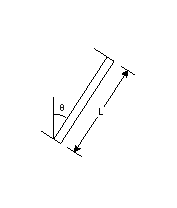
\includegraphics[width=0.5\linewidth, trim=0 20 0 20, clip]{Figures/inclined_plate.pdf}
    \caption{Inclined photovoltaic module. Adapted from \cite{Cengel2014NaturalConvection}}
    \label{fig:inclined_plate}
\end{figure}

Thus, Equation \ref{eq:rayleigh_number_tilted_function} is the appropriate mathematical expression for the Rayleigh number of a tilted photovoltaic module, $\text{Ra}_\theta$. \cite{Cengel2014NaturalConvection}.

\begin{equation}
    \text{Ra}_\theta = \frac{g\sin(\theta)\beta(T_s-T_\infty)L_c^3}{\nu\alpha}
    \label{eq:rayleigh_number_tilted_function}
\end{equation}

A casual inspection of Equation \ref{eq:rayleigh_number_tilted_function} indicates that the Rayleigh number for a tilted photovoltaic module, $\text{Ra}_\theta$, is directly proportional to the tilt angle, $\theta$, within the range of $0^\circ$ to $60^\circ$ \cite{Cengel2014NaturalConvection}. Therefore, increasing the tilt angle within this range results in a corresponding increase in the Rayleigh number.\vspace{0.5em}

The Nusselt number, $\text{Nu}$, is the ratio of convective to conductive heat transfer. \cite{Basu2019MassMeter} For simple empirical correlations in natural convection, an exponential relationship exists between the average Nusselt number, $\text{Nu}$, and the relevant Rayleigh number, shown in Equation \ref{eq:avg_nusselt_number_natural_convection} \cite{Cengel2014NaturalConvection}.

\begin{equation}
    \text{Nu} = C\,\text{Ra}_\theta^n
    \label{eq:avg_nusselt_number_natural_convection}
\end{equation}

Therefore, the increase in the Rayleigh number leads to an increase in the Nusselt number. Moreover, Equation \ref{eq:convective_heat_transfer_coefficient} reveals that an increase in the Nusselt number, $\text{Nu}$, causes an increase in the convective heat transfer coefficient, $h$. \cite{Cengel2014NaturalConvection}.
\begin{equation}
    h = \frac{\text{Nu} \times k}{L_c}
    \label{eq:convective_heat_transfer_coefficient}
\end{equation}

Finally, an inspection of Equation \ref{eq:rate_of_convective_heat_transfer_function} shows that an increase in the convective heat transfer coefficient, $h$, results in a higher convective heat transfer rate, $\dot{Q}_\text{conv}$, thereby supporting Abdulmunem et al.'s experimental findings. \cite{Cengel2014IntroductionConcepts} \vspace{0.5em}

However, while a vertical photovoltaic module improves natural convective heat transfer, it limits the surface area that is directly exposed to the sun, reducing power output. Thus, a tilt angle of $45^\circ$ from the horizontal axis (as in earlier NOCT testing \cite{InternationalElectrotechnicalCommission2005IECApproval}) is generally used in photovoltaic module testing because it represents more realistic conditions.\vspace{0.5em}

Natural convection-based cooling methods can effectively reduce an object's temperature; however, in photovoltaic modules, forced convection is significantly more efficient at transferring heat to the surroundings, resulting in greater improvements in module efficiency. A 2021 study led by A. Almuwailhi from King Saud University investigated the impact of both natural and forced convection cooling methods on the efficiency of photovoltaic modules. To promote natural convective heat transfer, Almuwailhi's team experimented with various channel air gaps. The most promising configuration featured an air gap height of $120$ mm, which led to a $1.2\%$ increase in photovoltaic module efficiency. For forced convection, Almuwailhi's team used airflow velocities of $2$ m/s and $3$ m/s. The results revealed a $3.8\%$ increase in efficiency with $2$ m/s airflow, and a $4\%$ increase with $3$ m/s airflow. \cite{Almuwailhi2023InvestigatingRiyadh} As a result, the remainder of this literature review will be dedicated to a comprehensive examination of forced convection cooling methods.

\subsubsubsection{Forced Convection and Relevant Cooling Methods} \label{sec:forced_convection_and_relevant_cooling_methods}
Forced convection is a mode of heat transfer in which fluid flow over a surface is induced by external means such as a fan, pump, or wind, rather than resulting from natural buoyancy forces. \cite{Cengel2014IntroductionConcepts} Figure \ref{fig:cooling_of_boiled_egg_forced_convection} illustrates how forced convective heat transfer can be applied to cool a hot egg.\par

\begin{figure}[ht]
    \centering
    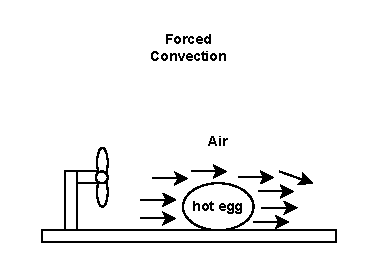
\includegraphics[width=0.5\textwidth, trim=0 5 0 10, clip]{Figures/cooling_of_boiled_egg_forced_convection.pdf}
    \caption{The cooling of a boiled egg by forced convection. Adapted from \cite{Cengel2014IntroductionConcepts}}
    \label{fig:cooling_of_boiled_egg_forced_convection}
\end{figure}

% - Explain a little bit more about forced convection and when you might consider natural convection, etc. (E.g., the relationship between the Reynold's number and the Grashof number.\vspace{0.5em}

Similar to natural convection, forced convection involves the development of velocity and thermal boundary layers that control momentum and heat transfer in the vicinity of the surface.\vspace{0.5em}

% Forced Convection Velocity Boundary Layer
\begin{figure}[H]
    \centering
    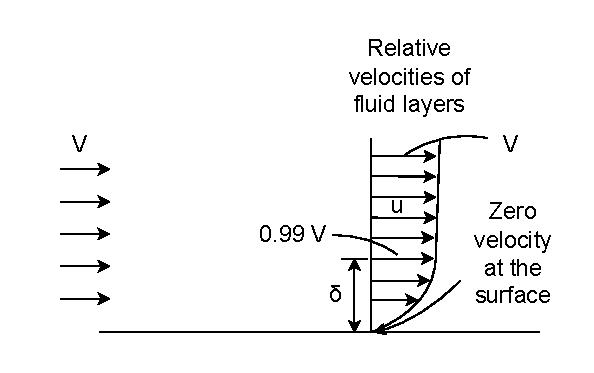
\includegraphics[width=0.6\linewidth]{Figures/velocity_boundary_layer.pdf}
    \caption{Velocity boundary layer over a flat plate. \cite{Cengel2014FundamentalsConvection}}
    \label{fig:velocity_boundary_layer}
\end{figure}

% No slip condition
Figure \ref{fig:velocity_boundary_layer} illustrates the velocity profile caused by parallel fluid flow over a flat plate. To understand this velocity profile, the fluid is modelled as a series of adjacent layers stacked on top of one another. The fluid particles in the layer closest to a solid surface are subject to the no-slip condition, which states that their velocity must match that of the boundary, resulting in zero relative motion between the fluid and the surface. Since photovoltaic modules remain stationary during operation, the fluid layer in direct contact with the surface has a velocity, $u$, of zero. \cite{Cengel2014FundamentalsConvection}\vspace{0.5em}

% Boundary layer 
The stationary fluid layer adjacent to the surface exerts frictional resistance on the fluid layer above it, reducing its velocity through shear interaction between layers moving at different speeds. This process propagates through successive fluid layers, each experiencing a reduction in momentum due to shear from the layer beneath, resulting in a velocity profile that increases with distance from the surface, but at a decreasing rate. At the boundary layer thickness, $\delta$, the plate has negligible effect on the velocity of the fluid. Thus, $\delta$, is typically defined as the distance from the surface where $u = 0.99V$. Therefore, the velocity boundary layer can be defined as the region of flow above the plate, bounded by $\delta$, where the effects of viscous shearing forces are significant. \cite{Cengel2014FundamentalsConvection}\vspace{0.5em}

% Forced Convection Thermal Boundary Layer
\begin{figure}[ht]
    \centering
    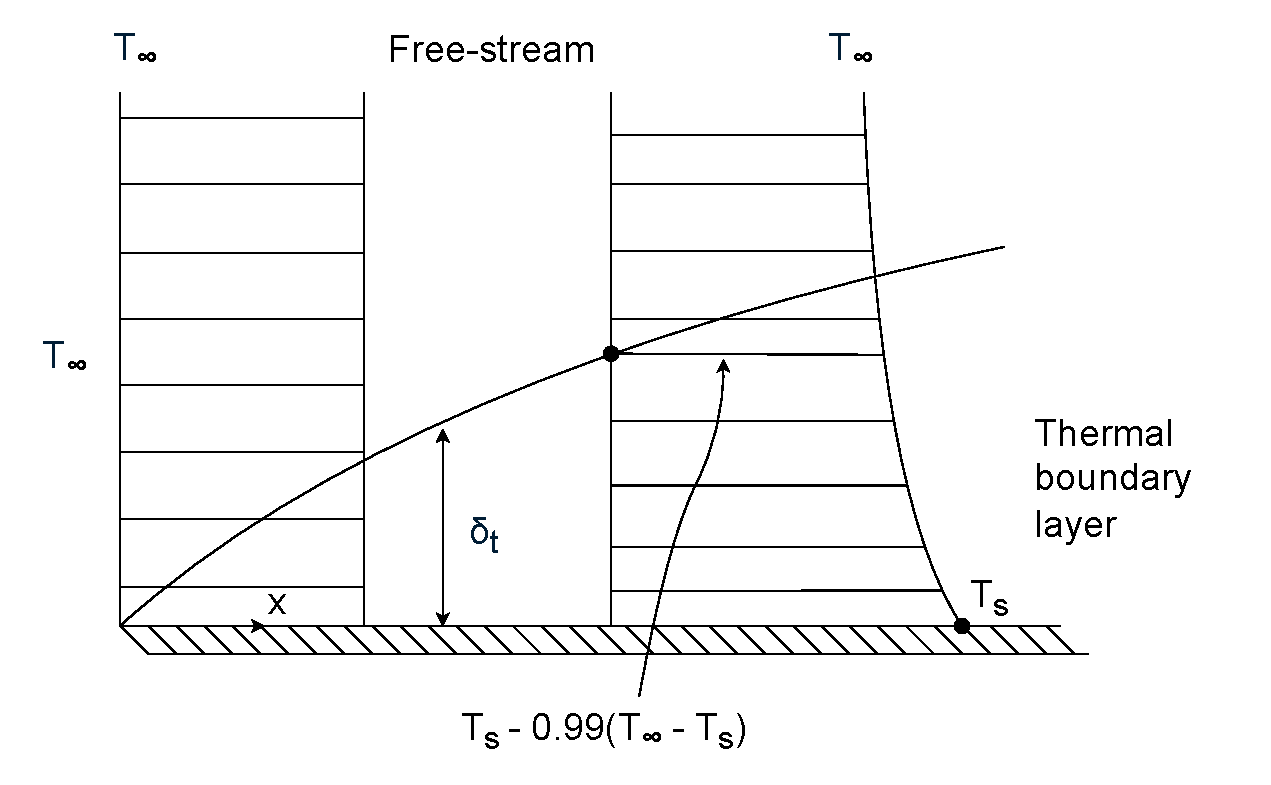
\includegraphics[width=0.7\linewidth]{Figures/thermal_boundary_layer.pdf}
    \caption{Thermal boundary layer on a flat plate (the plate surface is hotter than the fluid). Adapted from \cite{Cengel2014FundamentalsConvection}}
    \label{fig:thermal_boundary_layer}
\end{figure}

Figure \ref{fig:thermal_boundary_layer} shows the temperature profile that results due to the flow of parallel fluid over a flat plate. Given the focus on reducing photovoltaic module temperature, it is appropriate to illustrate a thermal boundary layer diagram where the plate surface is at a higher temperature than the surrounding fluid.\vspace{0.5em}

The fluid particles adjacent to the surface of the plate reach thermal equilibrium with the plate, adopting a temperature, $T_s$. This fluid layer transfers energy to the layer directly above it, resulting in a temperature gradient where each successive layer has a slightly lower temperature than the previous one, with the rate of decrease diminishing progressively. The boundary layer thickness, $\delta_t$, represents the perpendicular distance from the flat plate at which the influence of the plate's temperature, $T_s$, on the fluid temperature, $T_\infty$, becomes negligible. Thus, the thickness of the thermal boundary layer at any location on the surface occurs when $T = T_s-0.99(T_s-T_\infty)$. Therefore, the thermal boundary layer is defined as the flow region above the surface, bounded by $\delta_t$, where the temperature variation in the direction normal to the surface is significant. \cite{Cengel2014FundamentalsConvection}\vspace{0.5em}

A thicker thermal boundary layer results in a more gradual temperature gradient at the surface, reducing the effectiveness of convective cooling. To overcome this limitation, forced convection techniques are employed to disrupt and thin the boundary layer, enhancing the temperature gradient at the surface. This increase in gradient leads to a higher convective heat transfer rate, which lowers the operating temperature of the photovoltaic module and subsequently improves its efficiency.\vspace{0.5em}

% RCM: Air
In 2024, a study led by I. Al-Masalha from Al-Balqa Applied University investigated the enhancement of photovoltaic module efficiency through various cooling techniques, including air fans, water sprinklers, and hybrid systems. One of the approaches involved directing airflow over the surface of the modules using air fans. This method resulted in a module temperature reduction ranging from $6\%$ to $26\%$, as shown in Figure \ref{fig:air_cooling_temperature_graph}. Correspondingly, this temperature decrease led to an improvement in electrical efficiency within the range of $0.44\%$ and $1.45\%$, as illustrated in Figure \ref{fig:air_cooling_efficiency_graph} \cite{Al-Masalha2024ImprovingSystems}.

\begin{figure}[ht]
    \centering
    \begin{minipage}[b]{0.45\linewidth}
        \centering
        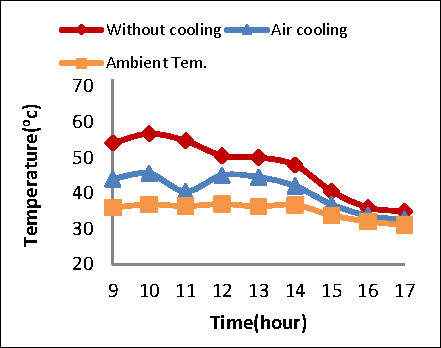
\includegraphics[width=\linewidth]{Figures/air_cooling_temperature_graph.pdf}
        \caption{Comparison of PV temperature when using air cooling over time. \cite{Al-Masalha2024ImprovingSystems}}
        \label{fig:air_cooling_temperature_graph}
    \end{minipage}
    \hfill
    \begin{minipage}[b]{0.45\linewidth}
        \centering
        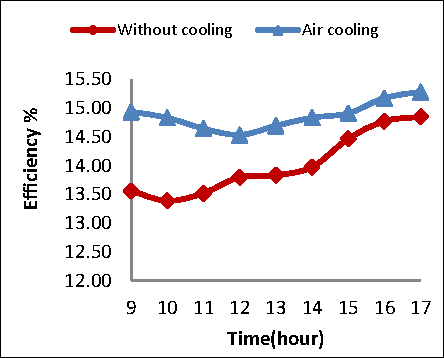
\includegraphics[width=\linewidth]{Figures/air_cooling_efficiency_graph.pdf}
        \caption{Comparison of efficiency when using air cooling over time. \cite{Al-Masalha2024ImprovingSystems}}
        \label{fig:air_cooling_efficiency_graph}
    \end{minipage}
\end{figure}

% RCM: Water
Al-Masalha et al.'s water cooling method involved spraying water directly onto the photovoltaic modules to dissipate heat. As illustrated in Figure \ref{fig:water_cooling_temperature_graph}, this technique resulted in a temperature reduction of the photovoltaic module ranging from $20.45\%$ to $35.44\%$. Consequently, as shown in Figure \ref{fig:water_cooling_efficiency_graph}, this temperature reduction led to an efficiency improvement between $0.6\%$ and $1.8\%$. \cite{Al-Masalha2024ImprovingSystems}

\begin{figure}[ht]
    \centering
    \begin{minipage}[b]{0.45\linewidth}
        \centering
        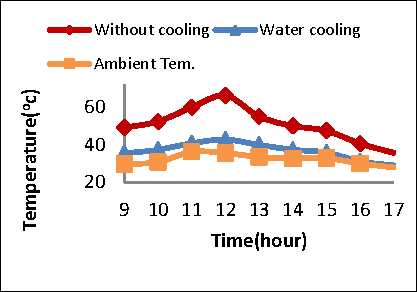
\includegraphics[width=\linewidth]{Figures/water_cooling_temperature_graph.pdf}
        \caption{Comparison of PV temperature when using water sprinklers over time. \cite{Al-Masalha2024ImprovingSystems}}
        \label{fig:water_cooling_temperature_graph}
    \end{minipage}
    \hfill
    \begin{minipage}[b]{0.45\linewidth}
        \centering
        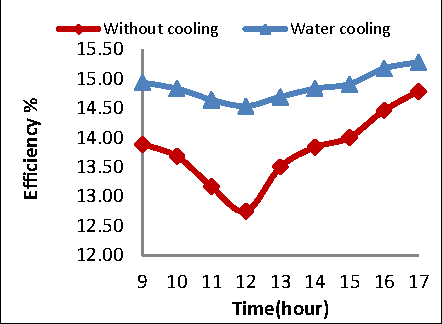
\includegraphics[width=\linewidth]{Figures/water_cooling_efficiency_graph.pdf}
        \caption{Comparison of efficiency when using water sprinklers over time. \cite{Al-Masalha2024ImprovingSystems}}
        \label{fig:water_cooling_efficiency_graph}
    \end{minipage}
\end{figure}

% RCM: Combined Cooling System
In their final approach, Al-Masalha's team developed a hybrid cooling system by combining water spraying and air cooling techniques. This integrated method produced the most significant results in terms of both temperature reduction and efficiency improvement. The hybrid cooling system achieved a temperature reduction in the range of $30\%$ and $40\%$, shown in Figure \ref{fig:hybrid_cooling_temperature_graph}. This substantial reduction in temperature led to an increase in photovoltaic module efficiency, ranging from $0.88\%$ to $2\%$, as illustrated in Figure \ref{fig:hybrid_cooling_efficiency_graph} \cite{Al-Masalha2024ImprovingSystems}.

\begin{figure}[H]
    \centering
    \begin{minipage}[b]{0.45\linewidth}
        \centering
        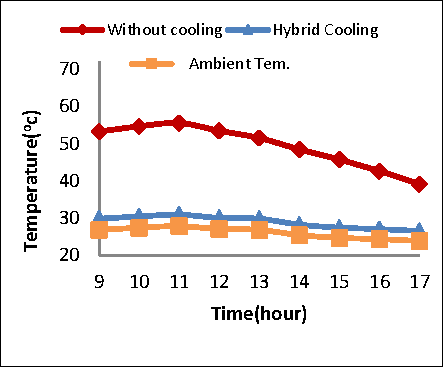
\includegraphics[width=\linewidth]{Figures/hybrid_cooling_temperature_graph.pdf}
        \caption{Comparison of PV temperature when using hybrid cooling over time. \cite{Al-Masalha2024ImprovingSystems}}
        \label{fig:hybrid_cooling_temperature_graph}
    \end{minipage}
    \hfill
    \begin{minipage}[b]{0.45\linewidth}
        \centering
        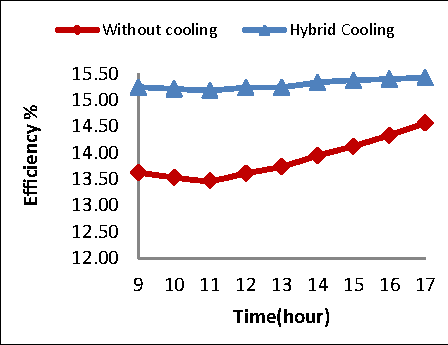
\includegraphics[width=\linewidth]{Figures/hybrid_cooling_efficiency_graph.pdf}
        \caption{Comparison of efficiency when using hybrid cooling over time. \cite{Al-Masalha2024ImprovingSystems}}
        \label{fig:hybrid_cooling_efficiency_graph}
    \end{minipage}
\end{figure}

% RCM: Nano-fluid
In recent times, nanofluid-based cooling methods have emerged as a highly effective technique for enhancing the thermal management and overall efficiency of photovoltaic modules. In 2022, T.K. Murtadha et al. conducted an experimental investigation into the performance enhancement of photovoltaic modules using titanium dioxide nanofluids. Their findings indicated that higher nanoparticle concentrations correlated with improved heat dissipation, resulting in a maximum efficiency gain of $19.23\%$ under optimal nanofluid cooling conditions. \cite{Murtadha2022ImprovingNanofluid}\vspace{0.5em}

% Explain why air is superior and then talk about VGs
The studies conducted by Al-Masalha et al. \cite{Al-Masalha2024ImprovingSystems} and Murtadha et al. \cite{Murtadha2022ImprovingNanofluid} clearly demonstrate that water and nanofluid cooling methods outperform air-based cooling in terms of thermal regulation and efficiency improvement for photovoltaic modules. However, despite their superior performance, water and nanofluid cooling systems are significantly less prevalent than air cooling in photovoltaic applications. This disparity is primarily due to several practical limitations. Both water and nanofluid systems entail higher initial and operational costs, as well as increased system complexity. \cite{Dwivedi2020AdvancedArt, Suresh2018RoleEfficiency} Additionally, they demand more frequent and intensive maintenance compared to air cooling systems, further escalating long-term expenses. \cite{Samykano2023HybridApplications, Ponticorvo2022FoulingFluid} Moreover, the structural load associated with liquid-based cooling is greater due to the added weight of the coolant medium, which imposes additional design and material constraints. \cite{Sakanova2016InvestigationAircraft} These factors collectively impact the cost-effectiveness of photovoltaic cooling strategies, rendering air cooling the most viable option for both commercial and residential implementations. Consequently, air cooling remains the most commonly employed method for photovoltaic module thermal management. \cite{Dwivedi2020AdvancedArt} \vspace{0.5em}

As was stated previously, Al-Masalha et al. implemented active cooling of photovoltaic modules using electric powered air fans to facilitate convective heat transfer. \cite{Al-Masalha2024ImprovingSystems} However, this approach incurs a parasitic energy cost, as external power is required to operate the fans. Vortex generators provide a passive cooling alternative that uses wind to induce localised turbulence and enhance convective heat transfer. Therefore, this literature review will examine the application of vortex generators in enhancing the thermal management of photovoltaic modules, ultimately leading to improved module efficiency.

\subsubsection{Vortex Generators}
\subsubsubsection{An Overview of Vortex Generator Effects on Heat Transfer Enhancement}
Vortex generators are protrusions on a heat transfer surface that induce swirling flow around an axis, creating vortices that enhance convective heat transfer. \cite{Awais2018HeatActivities} Figure \ref{fig:vortex_generator} depicts the interaction between fluid and a cylindrical vortex generator upon contact.

\begin{figure}[H]
    \centering
    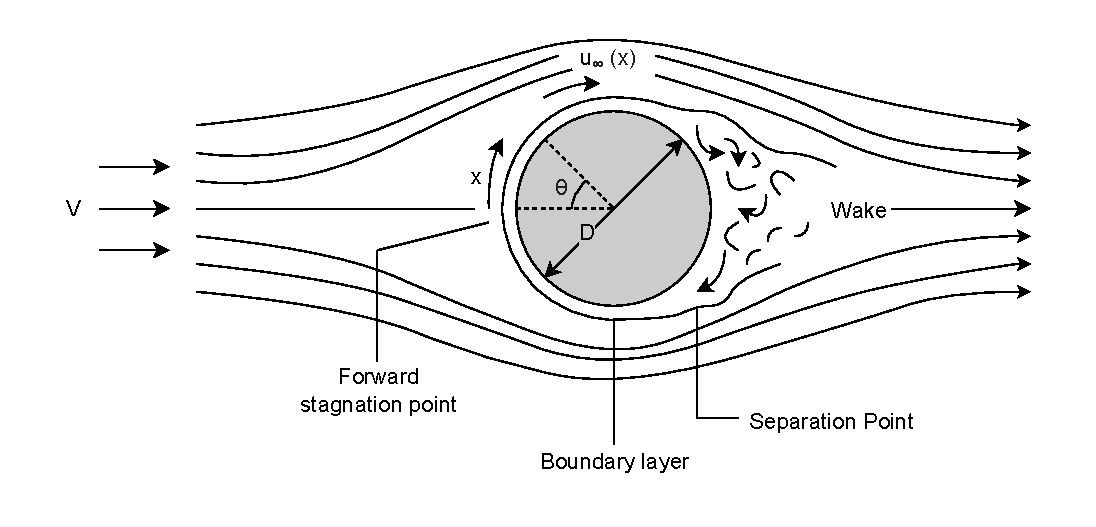
\includegraphics[width=1\linewidth,  trim=0 10 0 10, clip]{Figures/vortex_generator.pdf}
    \caption{Fluid flow over a cylinder. Adapted from \cite{VanTreuren2015ABSTRACTTurbines}}
    \label{fig:vortex_generator}
\end{figure}

Figure \ref{fig:vortex_generator} also illustrates two key features associated with vortex generators: the forward stagnation point and the separation point. At the forward stagnation point, the fluid velocity, $u$, is zero, while the separation point marks the location where the airflow detaches from the surface of the object. At the separation point, vortices, referred to as Kármán vortices in the context of cylindrical bodies, are generated. \cite{Wille1960KarmanStreets} These vortices promote mixing between the high-momentum outer fluid and the low-momentum near-wall fluid, enhancing momentum and energy exchange near the surface. This mixing leads to the thinning of the thermal boundary layer. As discussed in Section \ref{sec:forced_convection_and_relevant_cooling_methods}, an inverse relationship exists between the thermal boundary layer thickness and the rate of convective heat transfer. Therefore, the reduction in boundary layer thickness results in an enhanced convective heat transfer rate.

\subsubsubsection{Quantifying the Effect of Vortex Generators on Heat Transfer}
The location of the separation point on a cylinder depends on the boundary layer’s transition from laminar to turbulent flow. This transition is primarily characterised by the Reynolds number, \(\text{Re}_D\), which is defined as the ratio of inertial to viscous forces in the fluid. For cylindrical shapes, the Reynolds number is calculated using Equation~\ref{eq:reynolds_number}~\cite{Cengel2014ExternalConvection}.

\begin{equation}
    \text{Re}_D = \frac{\rho V D}{\mu} = \frac{V D}{\nu}
    \label{eq:reynolds_number}
\end{equation}

To estimate the average Nusselt number for cross flow over a cylinder, Churchill and Bernstein (1977) proposed an empirical correlation that accounts for the Reynolds and Prandtl numbers, as shown in Equation~\ref{eq:churchill_bernstein_average_nusselt_number}~\cite{Cengel2014ExternalConvection}.

\begin{equation}
    \text{Nu}_{\text{cyl}} = 0.3 + \frac{0.62\,\text{Re}^{1/2}\,\text{Pr}^{1/3}}{\left[1 + (0.4/\text{Pr})^{2/3}\right]^{1/4}} \left[1 + \left(\frac{\text{Re}}{282,000}\right)^{5/8}\right]^{4/5}
    \label{eq:churchill_bernstein_average_nusselt_number}
\end{equation}

Once the average Nusselt number is determined, the average convective heat transfer coefficient, \(h\), can be calculated using Equation~\ref{eq:average_nusselt_number_convective_heat_transfer_coefficient}~\cite{Cengel2014ExternalConvection}.

\begin{equation}
    \text{Nu}_{\text{cyl}} = \frac{h D}{k}
    \label{eq:average_nusselt_number_convective_heat_transfer_coefficient}
\end{equation}

Finally, the convective heat transfer coefficient can be used to determine the rate of convective heat transfer, as shown in Equation~\ref{eq:rate_of_convective_heat_transfer_function}. \cite{Cengel2014IntroductionConcepts} \vspace{0.5em}

In recent years, several studies have been published examining the influence of vortex generators on the rate of convective heat transfer. A 2024 study led by Z. Zhou from the University of New South Wales investigated the effect of vortex generators on photovoltaic module cooling. Zhou et al. attached rectangular wing vortex generators, made from either aluminium sheet or 3D printed thermally conductive polymer, to the rear side of the photovoltaic modules. Although the vortex generators were optimised for free convection, both designs successfully reduced the photovoltaic module temperature by $1.5^{\circ} \text{C}$ under low wind conditions and high irradiance. In scenarios with high module temperatures and windy conditions, the aluminium vortex generators achieved a greater cooling effect, reducing the module temperature by $2.5^{\circ} \text{C}$. \cite{Zhou2024Long-termCooling} \vspace{0.5em}

Zhou et al.'s observation of varying results due to different materials used in vortex generators demonstrates how modifications to vortex generator parameters can significantly impact their ability to reduce photovoltaic module temperature. \cite{Zhou2024Long-termCooling} As a result, various studies have investigated the influence of other vortex generator parameter modifications on the thermal performance of photovoltaic modules.

\subsubsubsection{Vortex Generators Orientation}
A 2023 study conducted by S. Schiffman from the University of New South Wales investigated the effect of vortex generator orientation on photovoltaic module temperature.\par
Schiffman oriented 3D printed vortex generators in a forward formation, shown in Figure ###, and in a backwards formation, shown in Figure ###.\cite{Schiffmann2023AnConditions}

\begin{figure}[H]
    \centering
    \begin{minipage}[b]{0.45\linewidth}
        \centering
        \includegraphics[width=\linewidth]{Figures/}
        \caption{Forward facing vortex generator configuration. Adapted from \cite{Schiffmann2023AnConditions}}
        \label{fig:fwd_full_fomation}
    \end{minipage}
    \hfill
    \begin{minipage}[b]{0.45\linewidth}
        \centering
        \includegraphics[width=\linewidth]{Figures/}
        \caption{Backward facing vortex generator configuration. Adapted from \cite{Schiffmann2023AnConditions}}
        \label{fig:back_full_formation}
    \end{minipage}
\end{figure}

Schiffman's experiment revealed that while both configurations facilitated cooling of the photovoltaic module, the forward facing configuration produced the most cooling, reducing the module's temperature by $1.82^\circ \text{C}$.\par

\subsubsubsection{Vortex Generators Shape}
\subsubsubsection{Vortex Generators Spacing}


\pagebreak
\subsection{Experimental Techniques}
\subsubsection{Infrared Thermography}
\subsubsection{Thermocouple Sensors}
\subsubsection{Particle Image Velocimetry}

\subsection{Literature Gap}
% \subsection{Energy Balance Maybe??? Depends on what we do for Charitha.}

\pagebreak


% \subsubsection{Cooling through Forced Convection}
% \begin{itemize}
%     \item What is forced convection?
%     \item How is forced convection used as a cooling method for photovoltaic modules?
%     \begin{itemize}
%         \item DC Fan Experiment
%         \item Floating Photovoltaic Module Experiment
%     \end{itemize}
%     \item Are there drawbacks to forced convection as a cooling method for photovoltaic modules?
%     \item Air vs Water Cooling Experiment
%     \item Air Cooled Modified Photovoltaic Module Experiment
%     \item Single Fin vs Multiple Fin Experiment
% \end{itemize}

% \subsubsection{Cooling through Vortex Generators}
% \begin{itemize}
%     \item What is a vortex generator?
%     \item What is the purpose of vortex generators?
%     \item Examples of Vortex Generator Experiments in the Context of Photovoltaic Module Cooling
% \end{itemize}